\documentclass[xcolor=dvipsnames]{beamer}

\title[Modeling using Matchgates]{Generative Modeling using Matchgate Circuits}
\author{Peter Luo, Hong Ye Hu, Susanne F. Yelin}

\date{\today} 

\usetheme{Boadilla}
\usecolortheme{seahorse}
\useoutertheme[subsection=false]{miniframes}  
\useinnertheme{circles}

\definecolor{logoBlue}{HTML}{003278}
\definecolor{blueDark}{HTML}{a3b6d4}
\definecolor{blueLight}{HTML}{e7eef8}
\definecolor{grey}{HTML}{b1b5b8}

\setbeamercolor*{palette tertiary}{bg=blueDark}
\setbeamercolor{frametitle}{fg=black,bg=blueLight}
\setbeamercolor{normal text}{fg=black,bg=white}

\usefonttheme{professionalfonts}
\usepackage{newpxtext}
\renewcommand\familydefault{\rmdefault}
\usepackage{amsmath}
\usepackage{bm}
\usepackage{tikz}
\usetikzlibrary{quantikz}
\usepackage{graphicx}

\DeclareMathOperator*{\E}{\mathbb{E}}

\begin{document}

\frame{\titlepage}

\section{Generative Modeling}

\begin{frame}{Neural Networks}

  \begin{itemize}
    \item Neural Networks are a means by which machine learning is carried out, and its architecture is inspired by neurons
  \end{itemize}
  \begin{figure}
    \centering
    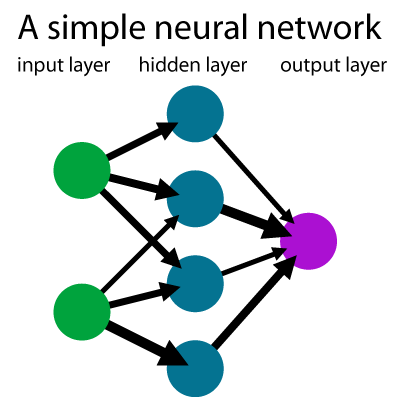
\includegraphics[width=0.4\textwidth]{NN.png}
  \end{figure}

\end{frame}

\begin{frame}{}
  \begin{itemize}
    \item Each neuron will output 
    $$f\left(b+\sum w_ix_i\right),$$
    where $f$ is an ``activation function'', the $w_i$ are the ``weights'', the $b$ is the ``bias'', and the $x_i$ being the inputs
  \end{itemize}
  \begin{figure}
    \centering
    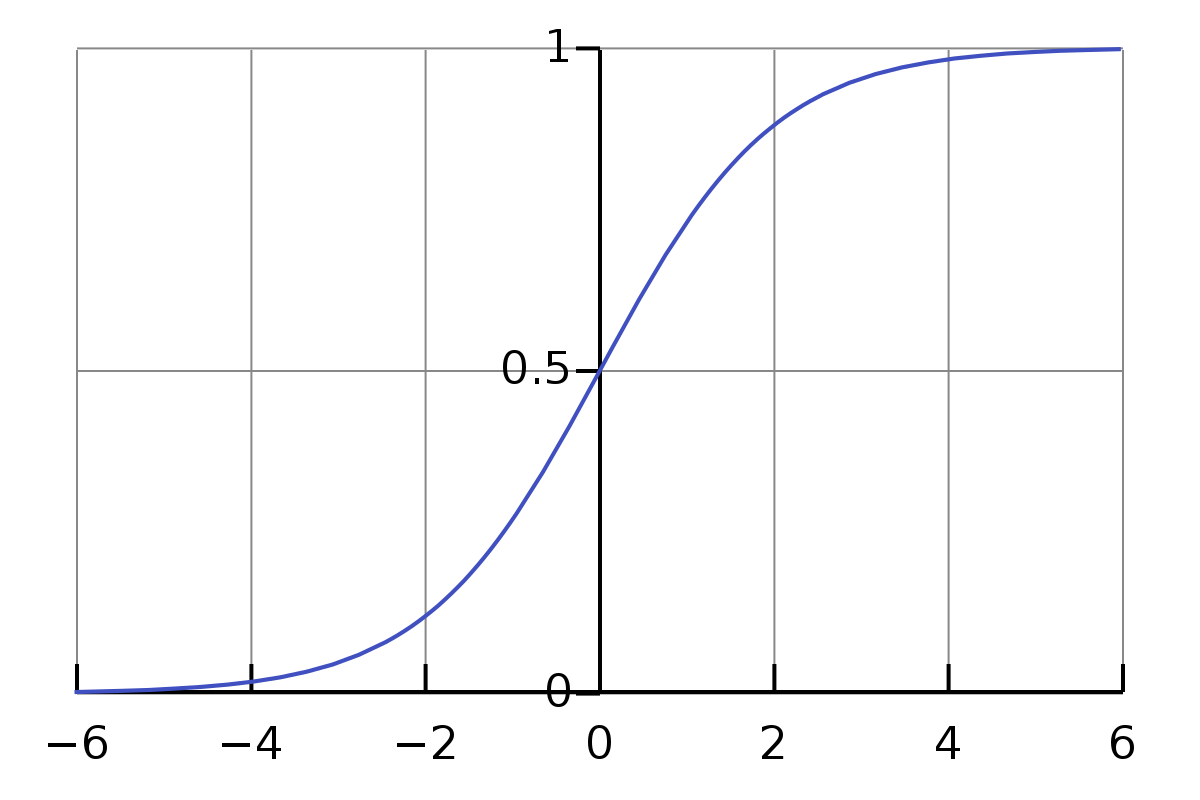
\includegraphics[width=0.55\textwidth]{sigmoid.png}
  \end{figure}

\end{frame}

\begin{frame}{How Neural Networks Learn}
  
  \begin{itemize}
    \item Define a ``\textcolor{red}{loss function}'' $L(\bm{w},\bm{b})$ which captures how close the network's output is to the desired output
  \end{itemize}

  \begin{figure}
    \centering
    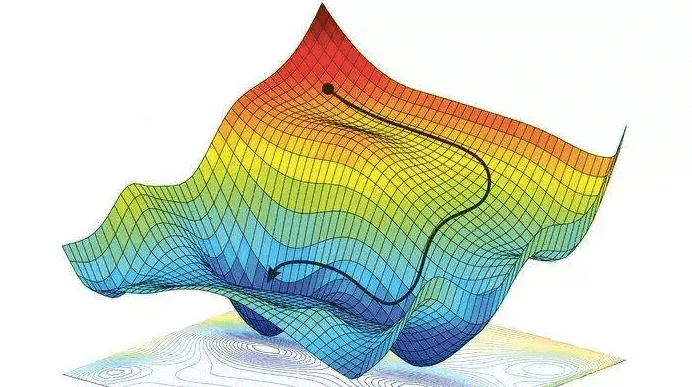
\includegraphics[width=0.5\textwidth]{gd.png}
  \end{figure}

  \begin{itemize}
    \item We can use optimization algorithms to adjust $\bm{w}$ and $\bm{b}$ to get closer and closer to the minimum of $L$ 
  \end{itemize}

\end{frame}

\begin{frame}{Generative Modeling}

    \begin{itemize}
      \item Rather than doing a classification or prediction task, generative models strive to generate more instances of their training data
      \item Examples: DALL-E, Voice Generators
      \item \textcolor{red}{Goal of this project:} To use a Matchgate circuit and the MNIST dataset to generate new images of handwritten digits
    \end{itemize}

    \begin{figure}
      \centering
          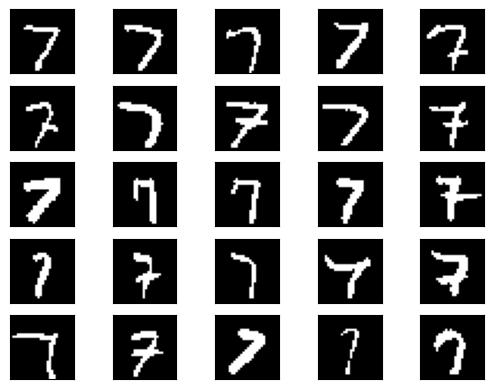
\includegraphics[width=0.4\textwidth]{MNIST.png}
      \end{figure}

\end{frame}

\begin{frame}{Generative Adversarial Networks (GAN)}

  \begin{itemize}
    \item Consists of two networks $G$ and $D$ with parameters $\bm{\theta}$ and $\bm{\phi}$ and their own loss functions $L_G(\bm{\theta},\bm{\phi})$ and $L_D(\bm{\theta},\bm{\phi})$
    \item $G:\{0,1\}^{28\times 28}\to\{0,1\}^{28\times 28}$ and $D:\{0,1\}^{28\times 28}\to [0,1]$
  \end{itemize}

  \begin{figure}
    \centering
    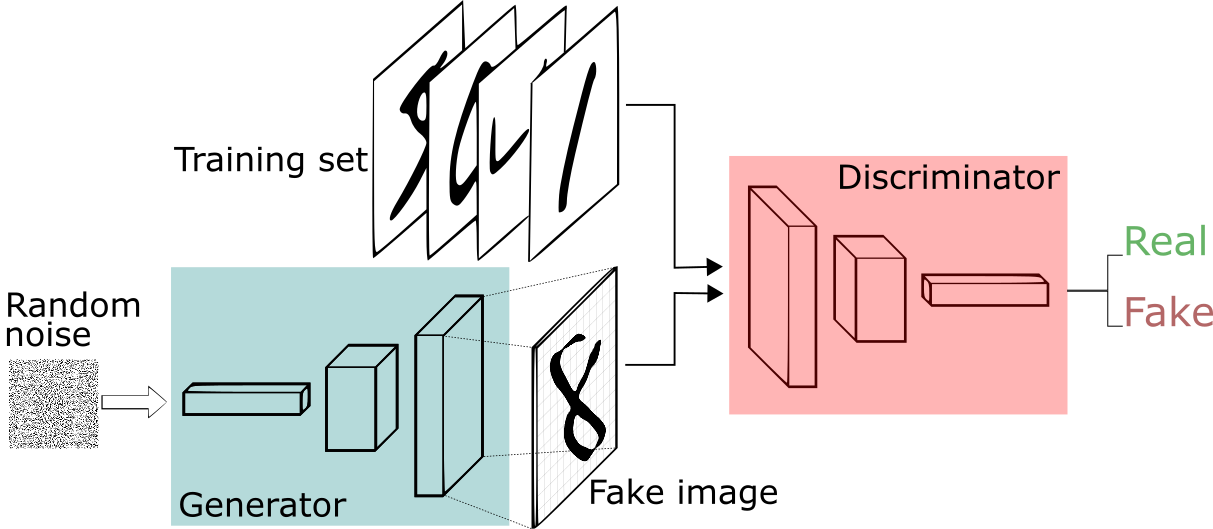
\includegraphics[width=0.7\textwidth]{GANs.png}
  \end{figure}

\end{frame}

\begin{frame}

  \begin{itemize}
    \item Assume that the real data $\bm{x}_1,\ldots,\bm{x}_n$ comes from an underlying probability distribution $p_{\text{real}},$ and recall that the input to $G$ are samples $\bm{z}_1,\ldots,\bm{z}_n$ from $p_{\text{prior}}$
    \item The loss functions are 
    \begin{align*}
      L_G(\bm{\theta},\bm{\phi})&=-\E_{\bm{z}\sim p_{\text{prior}}}\left[\log(D(G(\bm{z})))\right]\\
      L_D(\bm{\theta},\bm{\phi})&=-\left(\E_{\bm{x}\sim p_{\text{real}}}\left[\log(D(\bm{x}))\right]+\E_{\bm{z}\sim p_{\text{prior}}}\left[\log(1-D(G(\bm{z})))\right]\right).
    \end{align*}
  \end{itemize}

  \begin{figure}
    \centering
    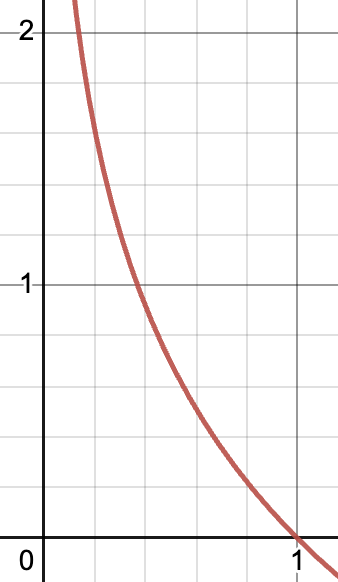
\includegraphics[width=0.15\textwidth]{neglog.png}
  \end{figure}

\end{frame}
  
\section{Quantum Machine Learning}

\begin{frame}{Quantum Computing}
  
  \begin{itemize}
    \item Leverages principles from quantum mechanics to do computations
    \item Consequently, it can solve certain problems exponentially faster than classical computers, reducing runtime from millions of years to just a few minutes
    \item It can also break some commonly used encryption methods, such as RSA or ECC
    \item It can simulate molecular interactions efficiently, which has implications in drug discovery and the material sciences
  \end{itemize}

\end{frame}

\begin{frame}{Limitations}

  \begin{itemize}
    \item Quantum computers need to be kept at very cold temperatures, thus requiring a large amount of energy
    \item Real quantum devices are noisy
    \item Number of qubits that we're able to run on the best quantum computers is relatively small (on the order of $10^2$)
    \item A lot is known about what is \textcolor{red}{theoretically possible}, but not a lot is known about their actual performance 
    \item Temporary solution: classical simulation 
  \end{itemize}
  
\end{frame}

\begin{frame}{Quantum Computing}

  \begin{minipage}[t]{0.48\linewidth}
      Classical computing:
      \begin{itemize}
          \item Consists of logic gates (e.g. AND, NOT, OR)
          \item One classical bit: a $0$ or a $1$
      \end{itemize}
  \end{minipage}
  \hfill
  \begin{minipage}[t]{0.48\linewidth}
      Quantum computing:
      \begin{itemize}
          \item Consists of quantum gates, represented by unitary matrices with complex entries
          \item One quantum bit: a vector of two complex numbers, which describes the probability of being measured in the $0$ or $1$ state
      \end{itemize}
  \end{minipage}

\end{frame}

\begin{frame}{Quantum Bits}
  \begin{itemize}
    \item One qubit looks like 
    $$a\ket{0}+b\ket{1}\to
    \begin{pmatrix}
      a\\
      b
    \end{pmatrix}$$
    \item $|a|^2$ and $|b|^2$ are the probabilities so we require $|a|^2+|b|^2=1$
    \item For two qubits,  
    $$a\ket{00}+b\ket{01}+c\ket{10}+d\ket{11}\to
    \begin{pmatrix}
      a\\
      b\\
      c\\
      d
    \end{pmatrix}$$
    \item The number of complex numbers we need to keep track of scales \textcolor{red}{exponentially} with the number of qubits
    \item Quantum computers are hard to simulate classically
  \end{itemize}
\end{frame}

\begin{frame}{Quantum Gates}
  \begin{itemize}
    \item An $n$-qubit gate is a $2^n\times 2^n$ unitary matrix with complex entries
    \item A matrix $U$ is unitary if $UU^\dagger=I,$ where $\dagger$ means the conjugate transpose
    \item 1-qubit examples:
    $$H=\frac{1}{\sqrt{2}}
    \begin{pmatrix}
      1 & 1\\
      1 & -1
    \end{pmatrix},\qquad
    \begin{pmatrix}
      1 & 0\\
      0 & i
    \end{pmatrix},\qquad 
    \begin{pmatrix}
      \cos(\theta/2) & -\sin(\theta/2)\\
      \sin(\theta/2) & \cos(\theta/2)
    \end{pmatrix}
    $$
    \item Example:
    $$H\ket{0}=\frac{1}{\sqrt{2}}
    \begin{pmatrix}
      1 & 1\\
      1 & -1
    \end{pmatrix}
    \begin{pmatrix}
      1\\
      0
    \end{pmatrix}=
    \begin{pmatrix}
      1/\sqrt{2}\\
      1/\sqrt{2}
    \end{pmatrix}\to\frac{1}{\sqrt{2}}\ket{0}+\frac{1}{\sqrt{2}}\ket{1}$$
    \item To simulate quantum computers is to do matrix multiplications
  \end{itemize}
\end{frame}

\begin{frame}
  \frametitle{Parametrized Quantum Circuit}
  \begin{itemize}
    \item Quantum gates can be \textcolor{red}{parametrized}
    \item By replacing the neural network with a parametrized quantum circuit and then measuring its output, we obtain a \textcolor{red}{hybrid} quantum-classical system compatible with machine learning procedures
  \end{itemize}
  \begin{figure}
    \centering
    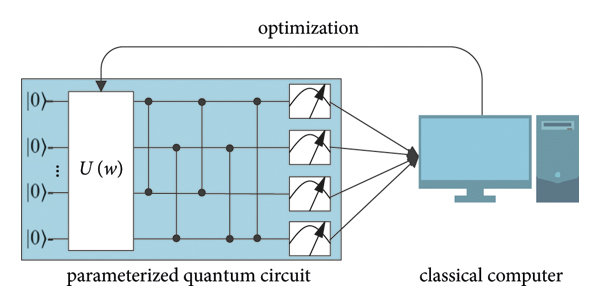
\includegraphics[width=0.7\textwidth]{pqc.png}
  \end{figure}
\end{frame}

\begin{frame}{Computing Gradients}
  \begin{itemize}
    \item Parameter-Shift Rule
    \item If $L(\bm{\theta})$ is the expectation value of some quantity with respect to the output of a quantum circuit with gates of the form $U_G(\bm{\theta})=e^{-ia\theta G}$ where $G^2=I,$ then
    \[\frac{\partial L}{\partial\bm{\theta}_i}=r\left(L\left(\bm{\theta}+\frac{\pi}{4r}\vec{\bf{e}}_i\right)+L\left(\bm{\theta}-\frac{\pi}{4r}\vec{\bf{e}}_i\right)\right)\]
    \item Proof uses 
    \[U_G(\theta)=e^{-i\theta G}=I\cos\theta-iG\sin\theta\]
    and 
    \[\frac{d}{d\theta}U_G(\theta)=-iGe^{-i\theta G}=-iGU_G(\theta)\]
  \end{itemize}
\end{frame}

\section{Matchgate Circuits}

\begin{frame}{Matchgates}
  \begin{itemize}
    \item Matchgates are a restricted class of parametrized quantum gates, generated by 
    $$e^{-iX\otimes X\theta/2},\quad e^{-iY\otimes Y\theta/2},\quad e^{-iX\otimes Y\theta/2},\quad e^{-iY\otimes X\theta/2},\quad e^{-iZ\theta/2}$$
    \item Matchgates are \textcolor{red}{differentiable} with respect to $\theta$ and can be simulated in \textcolor{red}{polynomial time} 
  \end{itemize}

  \begin{figure}
    \centering
    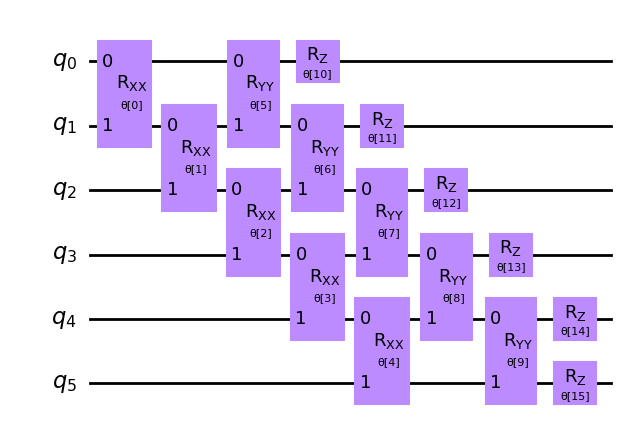
\includegraphics[width=0.5\textwidth]{output.png}
  \end{figure}

\end{frame}

\begin{frame}{Valiant's Definition}
  \begin{itemize}
    \item Matchgates were first introduced by Valiant (2001)
    \item For a given undirected weighted graph $G$ wher $V(G)=[n],$ define the \textcolor{red}{Pfaffian} to be
    \[\text{Pf}(B)=\sum_{\substack{\text{perfect matchings} \\ M}}\text{sgn}(M)\prod_{(ij)\in M}w_{ij},\]
    where $B$ is the adjacency matrix of $G$
    \item Theorem (Cayley): $\text{Pf}(B)^2=\text{Det}(B)$
    \item Pfaffians are computable in polynomial time
  \end{itemize}
\end{frame}

\begin{frame}
  \begin{itemize}
    \item Define the \textcolor{red}{Pfaffian sum} to be 
    \[\text{PfS}(B)=\sum_{A\subseteq [n]}\left(\prod_{i\in A}\lambda_i\right)\text{Pf}(B[A])\]
    \item Pfaffian sums are just Pfaffians:
    \[\text{PfS}(B)=
    \begin{cases}
      \text{Pf}(B+\Lambda_n) & n\text{ even}\\
      \text{Pf}(B^++\Lambda_{n+1}) & n\text{ odd}
    \end{cases}\]
    where
    \[\Lambda_n=
    \begin{pmatrix}
      0 & \lambda_1\lambda_2 & -\lambda_1\lambda_3 & \cdots\\
      -\lambda_1\lambda_2 & 0 & \lambda_2\lambda_3 & \cdots\\
      \lambda_1\lambda_3 & -\lambda_2\lambda_3 & \ddots & \\
      \vdots & \vdots & & 
    \end{pmatrix}\]
  \end{itemize}
\end{frame}

\begin{frame}
  \begin{itemize}
    \item A \textcolor{red}{matchgate} $\Gamma$ is $(G,X,Y,T)$ where $G$ is a graph and $X,Y,T$ partition the vertices. For $Z\subseteq X\cup Y,$ define 
    \[\chi(\Gamma,Z)=\mu(\Gamma,Z)\text{PfS}(G-Z)\]
    \item The \textcolor{red}{character matrix} $\chi(\Gamma)$ is the $2^{|X|}\times 2^{|Y|}$ matrix with 
    \[\chi(\Gamma)_{i,j}=\chi(\Gamma,X_i\cup Y_j).\]
    \item Defined in this way, not all matchgates are unitary
    \item Take the ones that are unitary and interpret them as quantum gates
    \item For a Matchgate circuit $C,$ 
    \[|\bra{\underline{y}}C\ket{\underline{x}}|^2=|\text{PfS}(M_{\underline{x},\underline{y}})|^2.\]
  \end{itemize}
\end{frame}

\begin{frame}{Matchgate Speedup}
  \begin{itemize}
    \item Valiant: Computing Pfaffians is fast
    \item Terhal and DiVincenzo (2001): There is a correspondence to noninteracting fermions in 1D, and computing determinants is fast
  \end{itemize}
\end{frame}

\section{Putting it all together}

\begin{frame}{Setup}
  \begin{enumerate}
    \item Use a parametrized quantum circuit made of matchgates as our $G$
    \item Use a classical neural network as $D$
    \item Train it just like you would train a GAN, i.e. use the same loss functions
  \end{enumerate}
  \begin{figure}
    \centering
    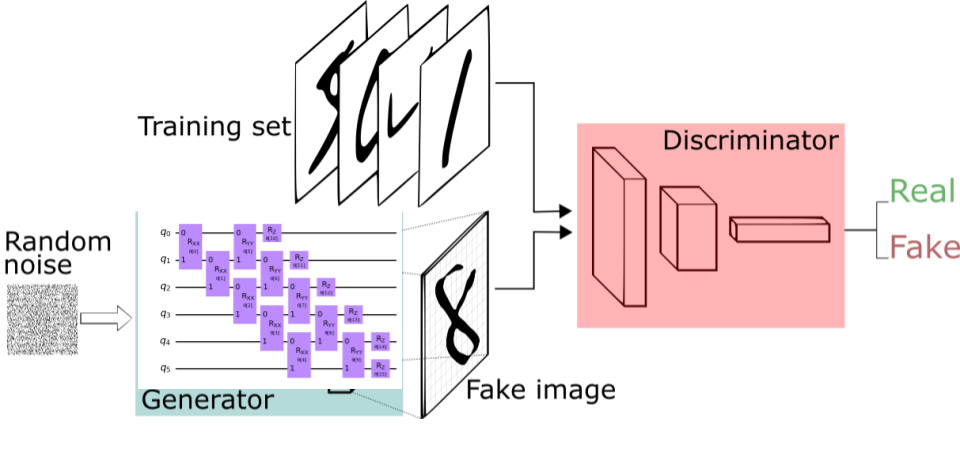
\includegraphics[width=0.7 \textwidth]{setup.png}
  \end{figure}
  \begin{itemize}
    \item Goal: Understand the performance of QML on a real dataset with a large number of qubits
  \end{itemize}
\end{frame}

\begin{frame}{Code}
  \begin{itemize}
    \item Written in Julia, using Yao package
    \item Utilized FLOYao package to harness Matchgate optimizations
    \item Current progress
  \end{itemize}
\end{frame}

\begin{frame}{Acknowledgements}
  \begin{itemize}
    \item Hong-Ye Hu and Susanne Yelin  
  \end{itemize}
  \begin{figure}[ht]
    \centering
    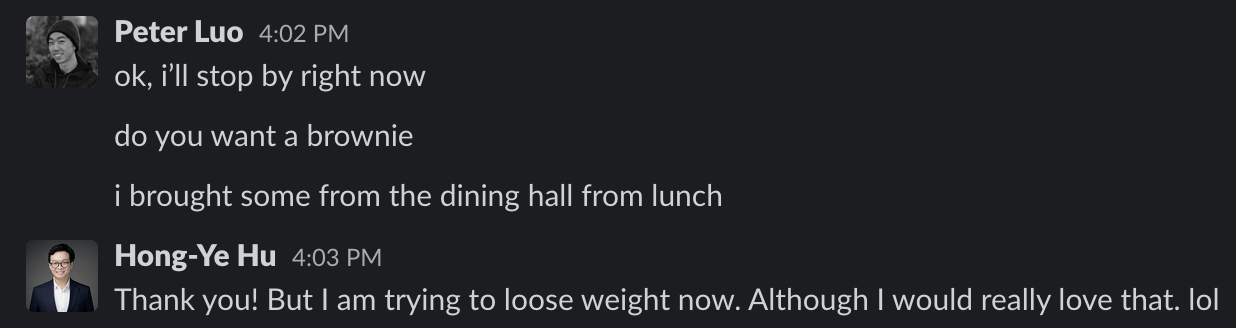
\includegraphics[width=0.8\textwidth]{HongYe.png}

    \centering
    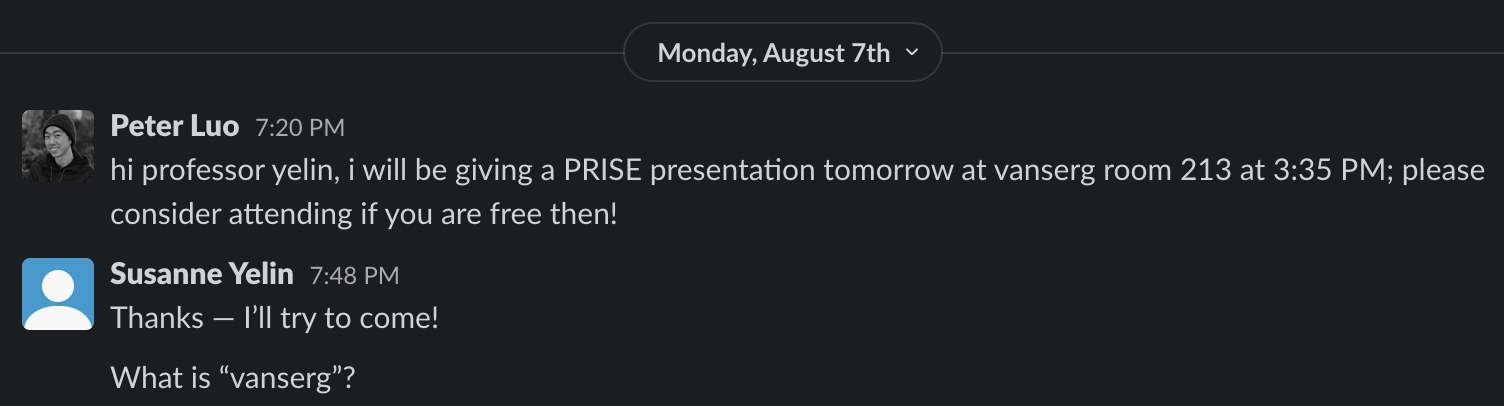
\includegraphics[width=0.8\textwidth]{Yelin.png}
  \end{figure}
\end{frame}

\begin{frame}
  \begin{itemize}
    \item Yelin group undergrads: Jorge, Fiona, Victoria, and Kevin
  \end{itemize}
  \begin{figure}
    \centering
    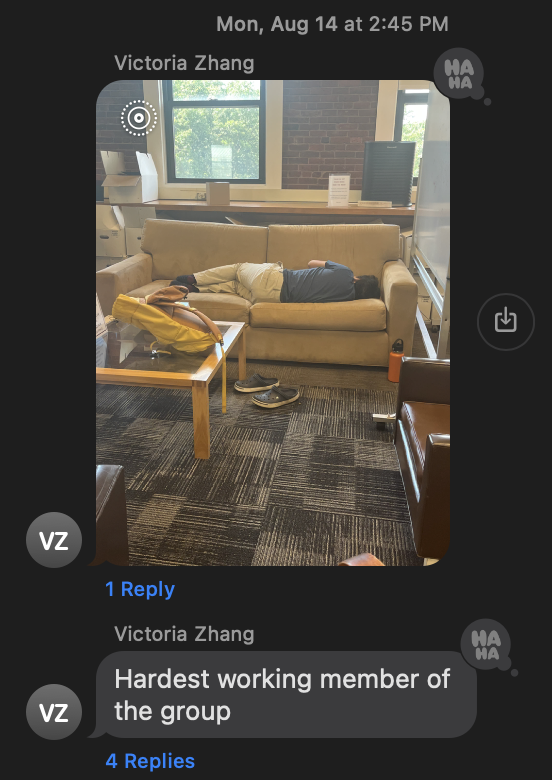
\includegraphics[width=0.32\textwidth]{Jorge.png}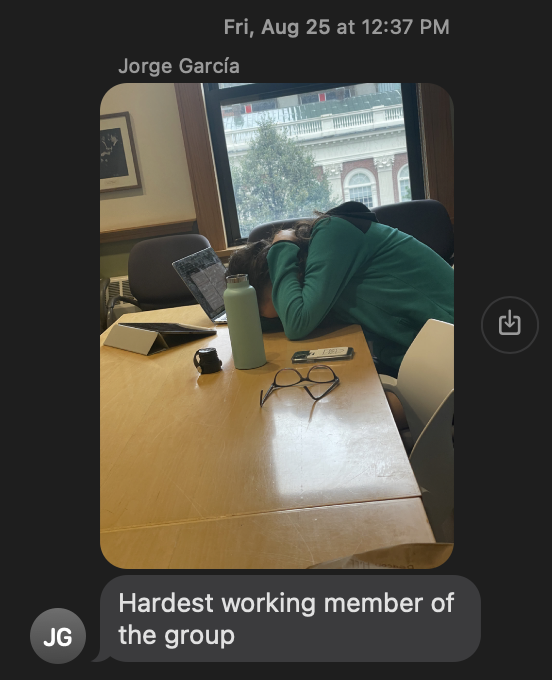
\includegraphics[width=0.32\textwidth]{Fiona.png} 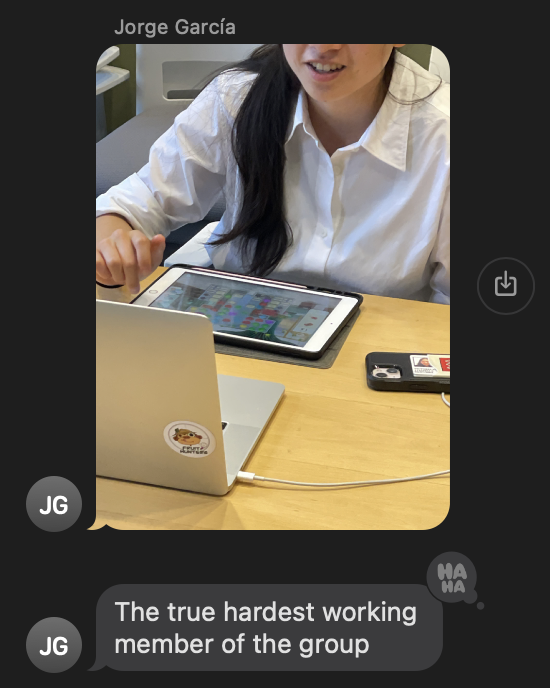
\includegraphics[width=0.32\textwidth]{Victoria.png}
  \end{figure}
\end{frame}

\begin{frame}{Questions?}
  
  \begin{figure}
    \centering
    
\includegraphics[width=0.5\textwidth]{thumbsup.png}
  \end{figure}

\end{frame}

\end{document}